% Dies ist Teil der Vorlesung Physik auf dem Computer, SS 2012,
% Axel Arnold, Universitaet Stuttgart.
% 
% Dieses Werk ist unter einer Creative Commons-Lizenz vom Typ
% Namensnennung-Weitergabe unter gleichen Bedingungen 3.0 Deutschland
% zugänglich. Um eine Kopie dieser Lizenz einzusehen, konsultieren Sie
% http://creativecommons.org/licenses/by-sa/3.0/de/ oder wenden Sie sich
% schriftlich an Creative Commons, 444 Castro Street, Suite 900, Mountain
% View, California, 94041, USA.

\chapter{Numerisches Differenzieren und Integrieren}

In diesem Kapitel geht es darum, wie eine Funktion, die an diskreten
Stützstellen gegeben ist, numerisch differenziert und integriert
werden kann. Die Grundlagen dazu wurden bereits mit dem Kapitel
``Darstellung von Funktionen'' gelegt: für die numerische Ableitung
liegt es nahe, aus der Taylorentwicklung geeignete Ausdrücke für die
Ableitungen zu gewinnen, und für die Integration bieten sich das
interpolierende Polynom oder auch ein Spline and, die sich mit dem
Computer leicht analytisch integrieren lassen.

Numerisches Integrieren und Differenzieren kann dabei nicht nur dazu
dienen, Integrale oder Ableitungen abzuschätzen, sondern erlaubt auch,
einfache Differential- oder Integralgleichungen numerisch zu
lösen. Dazu muss die Gleichung mit Hilfe der hier vorgestellten
Verfahren diskretisiert und das resultierende lineare Gleichungssystem
gelöst werden.

\section{Numerisches Differenzieren}
\index{Differenzieren}

Die erste Ableitung einer Funktion $f\in C^1([a,b])$ ist definiert als
\begin{equation}
  \lim_{h\to 0} \frac{f(x+h) - f(x)}{h}.
\end{equation}
Um den Grenzwert abzuschätzten, liegt es nahe, die Ableitung durch die
dividierte Differenz
\begin{equation}
  f'(\xi) \approx f[x,y] := \frac{f(x) - f(y)}{x - y}
\end{equation}
anzunähern, wobei $x$ und $y$ beide nahe bei $\xi$ liegen sollten.

Doch an welchem Punkt $\xi$ ist diese Näherung optimal? Gemäß
Mittelwertsatz gilt auf jeden Fall $f[x,y]=f'(\xi)$ für ein $\xi\in
[x,y]$. Man erwartet daher, dass $f[x,y]$ am besten in der
Intervallmitte $m=\frac{x+y}{2}$ approximiert. Das ist tatsächlich so,
wie wir nun per Taylorentwicklung sehen werden. Mit Entwicklung um $m$
und $h=x-y$ gilt
\begin{align}
  \frac{f(x) - f(y)}{x-y} &= \frac{1}{h}
  \biggl(+f(m) + \frac{h}{2}f'(m) + \frac{h^2}{8}f''(m) + \O(h^3)\nonumber\\
  &\phantom{= \frac{1}{h}\biggl(}-f(m) + \frac{h}{2}f'(m) - \frac{h^2}{8}f''(m) + \O(h^3)
  \biggr)\nonumber\\
  &=  f'(m) + \O(h^2).
\end{align}
Bei Ansatzpunkt $x$ gilt hingegen nur
\begin{align}
  \frac{f(x) - f(y)}{x-y} = \frac{1}{h}
  \biggl(f(x) + h f'(x) + \frac{h^2}{8}f''(x) + \O(h^3) - f(x) \biggr)
  =  f'(x) + \O(h).
\end{align}

In der Praxis ist die Funktion meist an an äquidistanten Stützstellen
$x_i$ mit $x_{i+1}-x_i=h$ gegeben. Dann ist, wie oben gezeigt, die
beste Zweipunkt-Näherung für die Ableitung die zentrale Differenz
\begin{equation}
  \label{eq:2orderdiff}
  \frac{f(x_{i+1}) - f(x_{i-1})}{2h} = f[x_{i-1},x_{i+1}] = f'(x_i) + \O(h^2),
\end{equation}
während für die linken und rechten dividierten Differenzen gilt:
\begin{equation}
  \frac{f(x_{i+1}) - f(x_{i})}{h} = f[x_{i},x_{i+1}] = f'(x_i) + \O(h)
\end{equation}
bzw.
\begin{equation}
  \frac{f(x_{i}) - f(x_{i-1})}{h} = f[x_{i},x_{i-1}] = f'(x_i) + \O(h).
\end{equation}

\subsection{Näherungen höhererer Ordnung und höhere Ableitungen}

Mit Hilfe von Taylorentwicklungen lassen sich auch Näherungen mit mehr
Stützpunkten und für höhere Ableitungen entwickeln.  Wir betrachten
zum Beispiel die Punkte für $k=-2(1)2$, d.h.\ die 5 benachbarten
Punkte, und suchen Koeffizienten $c_k$ derart, dass
\begin{equation}
  c_2 f(x_{i+2}) + c_1 f(x_{i+1})  + c_0 f(x_i) + c_{-1}f(x_{i-1}) +
  c_{-2}f(x_{i-2}) = f'(x_i) + \O(h^5),
\end{equation}
unabhänging von der Form von $f$ und seiner Ableitungen. Durch
Einsetzen der Taylorentwicklung
\begin{equation}
  f(x + k h) = f(x) + k\, hf'(x) + k^2\,\frac{h^2}{2} f''(x_i) +
  k^3\,\frac{h^3}{6}f^{(3)}(x) + k^4\,\frac{h^4}{24}f^{(4)}(x) + \O(h^5)
\end{equation}
können wir nun die obige Gleichung auf beiden Seiten als Vielfache von
$f(x)$, $f'(x)$, $f''(x)$ usw.\ schreiben. Da unsere Koeffizienten
unabhängig von diesen sein sollen, müssen die Vorfaktoren vor diesen
auf beiden Seiten übereinstimmen. Diese sind, beginnend bei $f(x)$:
\begin{align}
  \label{eq:derivatives}
  c_{2} + c_{-2} + c_{-1} + c_1 + c_0 &= 0\nonumber\\
  h\left[2 (c_{2} - c_{-2})  + c_{1} - c_{-1}\right] &= 1\nonumber\\
  \frac{h^2}{2}\left[4(c_{2} + c_{-2})  + c_{1} + c_{-1}\right] &= 0\nonumber\\
  \frac{h^3}{6}\left[8 (c_{2} - c_{-2})  + c_{1} - c_{-1}\right] &= 0\nonumber\\
  \frac{h^4}{24}\left[16 (c_{2} + c_{-2}) + c_{1} + c_{-1}\right] &= 0.
\end{align}
Durch Lösen des Gleichungssystems folgt
\begin{equation}
  \label{eq:4orderdiff}
  -\frac{1}{12h} f(x_{i+2}) + \frac{2}{3h} f(x_{i+1})  - \frac{2}{3h} f(x_{i-1}) +
  \frac{1}{12h}f(x_{i-2}) = f'(x_i) + \O(h^4).
\end{equation}
Auf diese Weise lässt sich auch die höhere Güte der zentralen
Differenz verstehen: tatsächlich entspricht diese der optimalen
Näherung durch $x_{i-1}$, $x_i$  und $x_{i+1}$, nur dass aus
Symmetriegründen der Koeffizient zu $x_i$ verschwindet.

Um nun zum Beispiel die zweite Ableitung zu berechnen, lösen wir
\eqref{eq:derivatives}, allerdings mit einer 1 nicht in der zweiten,
sondern dritten Zeile. Das ergibt
\begin{equation}
  \label{eq:3order2diff}
  \frac{1}{h^2}\left(-\frac{1}{12} f(x_{i+2}) + \frac{4}{3} f(x_{i+1}) +
  \frac{5}{2} f(x_i)  + \frac{4}{3} f(x_{i-1}) -
  \frac{1}{12}f(x_{i-2})\right) = f''(x_i) + \O(h^3).
\end{equation}

Mit drei Stützpunkten ergibt sich die Näherung für die zweite
Ableitung analog als
\begin{multline}
  \label{eq:1order2diff}
  \frac{1}{h^2}\bigl(f(x_{i+1}) -
  2f(x_i)  + f(x_{i-1})\bigr) =
  \frac{\frac{f(x_{i+1}) - f(x_i)}{h}  -
    \frac{f(x_i) - f(x_{i-1})}{h}}{h}
  = f''(x_i) + \O(h).
\end{multline}
Die mittlere Form zeigt, dass sich diese einfachste Form der zweiten
Ableitung auch als dividierte Differenz der dividierten Differenzen
verstehen lässt. Technisch wird also die zweite Ableitung also einfach
in erster Ordnung aus der ersten Ableitung in erster Ordnung
bestimmt. Analog lässt sich jede $n$-te Ableitung aus $n+1$
benachbarten Stützstellen in erster Ordnung durch dividierte
Differenzen approximieren.

\subsection{Genauigkeit}

\begin{figure}
  \centering
  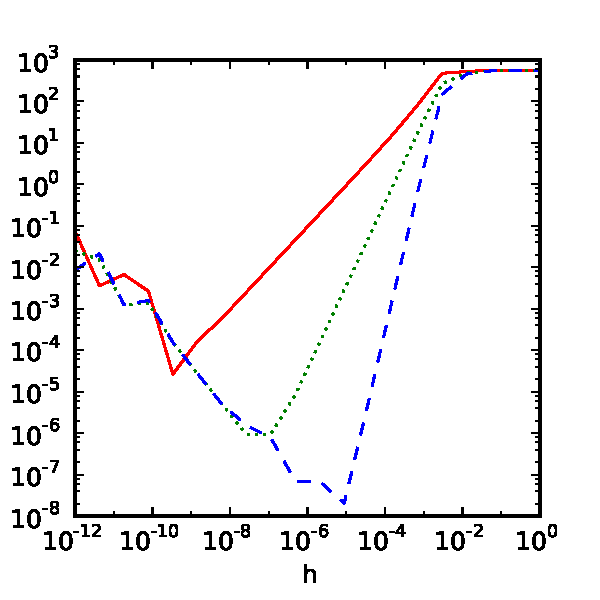
\includegraphics[width=0.5\textwidth]{plots/num_diff}
  \caption{Maximale Abweichung $\max_{x\in[-\pi,pi]} \abs{f'(x) - a(h;
      x)}$ für verschiedene Näherungen $a(h; x)$, als Funktion der
    Schrittweite $h$. Die Funktion ist $f(x)=sin(100x^2)$. Rot
    durchgezogen ist die linksseitige Differenz $a(h; x) = (f(x) -
    f(x-h))/h$, die zentrale Differenz $a(h; x) = (f(x+h) -
    f(x-h))/2h$ ist grün gepunktet und die Näherung 4. Ordnung
    \eqref{eq:4orderdiff} blau gestrichelt. Der rechtsseitige Abfall
    der Kurven entspricht den Ordnungen $\O(h)$ für die linksseitige
    Differenz, $\O(h^2)$ für die rechtsseitige und $\O(h^4)$ für die
    Gleichung 4. Ordnung. Das linksseitige Verhalten ist
    methodenunabhängig und durch die endliche Rechenauflösung bestimmt.}
  \label{fig:num_diff}
\end{figure}

Generell sind alle diese Näherungen numerisch instabil, da bei kleinen
Abständen $h$ auch $f(x)$ und $f(x+h)$ sehr ähnlich sind. Sind diese
betragsmäßig groß, kommt es zu Auslöschung, d.h., $f(x+h) - f(x)$ hat
deutlich weniger signifikante Stellen als Maschinengenauigkeit. Daher
gibt es stets ein optimales $h$, das allerdings von der unbekannten
zweiten Ableitung der betrachteten Funktion abhängt.

Auch Verfahren höherer Ordnung sind nicht notwendigerweise genauer, da
bei manchen Funktionen die Ableitungen sehr rasch wachsen. Dann ist
zwar $h^4$ sehr viel kleiner als $h^2$, aber der Vorfaktor
kompensiert das zunächst. Abbildung~\ref{fig:num_diff} illustriert
dieses Verhalten am Beispiel der Funktion $\sin(100x^2)$. Erst, wenn
die Schrittweite $h$ unter die charakteristische Breite von etwa 600
sinkt, spielt die Ordnung des Verfahrens eine Rolle. Wird allerdings
$h$ zu klein, zeigt sich die endliche Auflösung, mit der der Rechner
arbeitet, und der Fehler steigt wieder an.

\subsection{Beispiel: Besselsche Differentialgleichung}

\begin{figure}
  \centering
  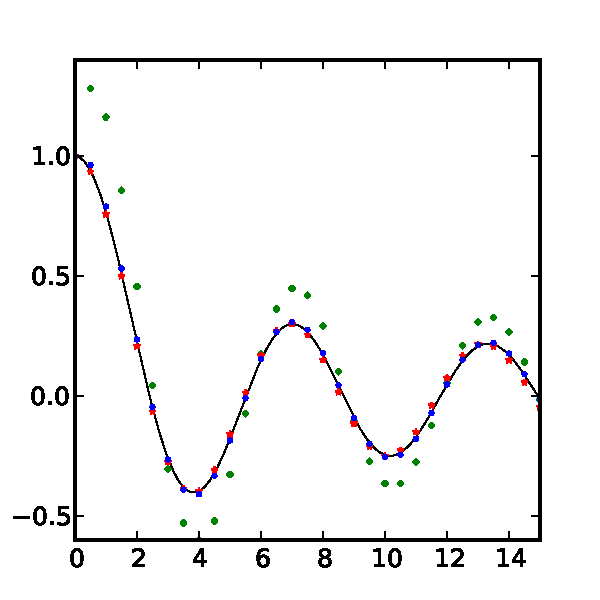
\includegraphics[width=0.5\textwidth]{plots/bessel_diff}
  \caption{Numerische Lösungen der Besselschen Differentialgleichung
    auf $[0,15]$ mit Schrittweite $h=0,5$ und $N=31$ Stützpunkten. Die
    durchgezogene schwarze Linie markiert die analytische Lösung. Mit
    grünen Diamanten ist die Lösung mit Hilfe von
    \eqref{eq:besseldiscrete} und Dirichletrandbedingungen
    dargestellt, für die roten Sterne wurden Funktionswert und
    Ableitung bei $0$ festgelegt. Blaue Punkte schließlich markieren
    den Löser dritter Ordnung mit Dirichletrandbedingungen, der von
    der analytischen Lösung praktisch nicht zu unterscheiden ist.}
  \label{fig:bessel_diff}
\end{figure}

Wir betrachten die Besselsche Differentialgleichung, eine gewöhnliche
lineare Differentialgleichung zweiter Ordnung:
\begin{equation}
  \label{eq:besselode}
  x^2\frac{d^2f}{dx^2} + x\frac{df}{dx} + (x^2-\nu)f = 0
\end{equation}
für $f\in C^{\infty}([0,\infty))$. Die Besselsche
Differentialgleichung spielt eine wichtige Rolle in der Physik, weil
sie den radialen Anteil der Laplacegleichung in Zylinderkoordinaten
beschreibt.  Für die Lösungen dieser Gleichung lassen sich schnell
konvergierende Reihen oder Integraldarstellungen
angeben~\cite{abramowitz70a,jackson99}, wir wollen aber zu
Demonstrationszwecken diese Differentialgleichung für $\nu=0$
numerisch lösen. Hierzu definieren wir $f_k := f(kh)$, $k\ge 0$, und
diskretisieren \eqref{eq:besselode} mit Hilfe der finiten Differenzen
\eqref{eq:2orderdiff} und \eqref{eq:1order2diff} in linearer Ordnung:
\begin{align}
  \label{eq:besseldiscrete}
  0 &= k^2\left(f_{k-1} - 2f_k + f_{k+1} \right)
  + k\left(\frac{1}{2} f_{k+1} - \frac{1}{2} f_{k-1}\right)
  + k^2h^2f_k\nonumber\\
  &= \left(k^2 - \frac{1}{2}k\right)f_{k-1}
  + k^2(h^2 - 2)f_k
  + \left(k^2 + \frac{1}{2}k\right)f_{k+1}.
\end{align}
Für die Lösung $f$ auf dem endlichen Intervall $[0, (N-1)h]$ sind das
$N-2$ Gleichungen, da zumindest für die Randpunkte die zweite
Ableitung so nicht abgeschätzt werden kann. Dies ist aber auch nicht
weiter verwunderlich, da wir ja die Randbedingungen noch nicht
festgelegt haben. Die natürlichen Randbedingungen der Diskretisierung
sind also Dirichlet-Randbedingungen, bei denen die fehlenden Randwerte
vorgegeben werden: $f_0 = f(0)=F_0$ und $f_{N-1} = f((N-1)h) = F_{N-1}$.

Wir erhalten das folgende lineare Gleichungssystem:
\begin{equation}
  \begin{pmatrix}
    1 & 0         & 0         &\ldots & \ldots & 0\\
    \nicefrac{1}{2} & -\lambda & \nicefrac{3}{2} & 0 & \ldots & 0\\
    0 & 3         & -4\lambda & 5 & 0\quad \ldots & 0\\
    & & \ddots & \ddots & \ddots\qquad\qquad \\
    0 & \ldots & 0 & \mu_n - \nu_n & -\mu_n\lambda & \mu_n + \nu_n\\
    0 &          &  \ldots  &   & 0      & 1
  \end{pmatrix}
  \begin{pmatrix}
    f_0\\
    \vdots\\
    f_{N-1}
  \end{pmatrix}=
  \begin{pmatrix}
    F_0\\
    0\\
    0\\
    \vdots\\
    0 \\
    F_{N-1}
  \end{pmatrix},
\end{equation}
wobei $\lambda=(2-h^2)$, $\mu_n=(N-2)^2$ und $\nu_n=
\frac{1}{2}(N-2)$. Die beiden äußeren Zeilen implementieren die
Dirichletbedingungen, die restlichen Zeilen Gleichung
\eqref{eq:besseldiscrete} für $k=1(1)N-1$.  Da die Matrix Bandstruktur
hat, können wir dieses lineare Gleichungssystem effizient mit dem
Gaußverfahren lösen.

Beispielcode~\ref{lst:bessel} zeigt ein Pythonskript zur Lösung dieses
Gleichungsssystems. Dessen Lösung für $h=0,5$ ist in
Abbildung~\ref{fig:bessel_diff} mit grünen Diamanten gezeigt und
weicht noch signifikant ab, was allerdings durch die hohe Schrittweite
bedingt ist. Mit einer Schrittweite $h < 0,1$ gäbe es keine sichtbaren
Abweichungen mehr.

Alternativ können wir statt der Dirichlet-Randbedingungen auch
Funktion $f(0) = F_0$ und Ableitung $f'(0)=F'_0$ am linken Rand
festlegen. Dann sieht das Gleichungssystem wie folgt aus:
\begin{equation}
  \begin{pmatrix}
    1 & 0         & 0         &\ldots & \ldots & 0\\
    -\nicefrac{1}{2h} & 0         & \nicefrac{1}{2h} &\ldots & \ldots & 0\\
    \nicefrac{1}{2} & -\lambda & \nicefrac{3}{2} & 0 & \ldots & 0\\
    0 & 3         & -4\lambda & 5 & 0\quad \ldots & 0\\
    & & \ddots & \ddots & \ddots\qquad\qquad \\
    0 & \ldots & 0 & \mu_n - \nu_n & -\mu_n\lambda & \mu_n + \nu_n\\
  \end{pmatrix}
  \begin{pmatrix}
    f_0\\
    \vdots\\
    f_{N-1}
  \end{pmatrix}=
  \begin{pmatrix}
    F_0\\
    F'_0\\
    0\\
    \vdots\\
    0 \\
  \end{pmatrix}.
\end{equation}
Abbildung~\ref{fig:bessel_diff} zeigt, dass die Lösung in diesem Fall
am linken Rand genauer ist, während sie zum rechten Rand hin
abweicht. Das ist ist zu erwarten, da unsere Bedingung die Lösung ja
nur am linken Rand zwingen, mit der analytischen Lösung
übereinzustimmen.

Generell zeigen allerdings sowohl Dirichlet- wie auch gemischte
Randbedingungen noch leichte Artefakte. Diese lassen sich durch
natürlich durch kleinere Schrittweite verringern, da die Lösung aber
$C^\infty$ ist, kann man aber stattdessen auch auf
Ableitungsnäherungen höherer Ordnung zurückzugreifen, etwa
\eqref{eq:3order2diff} und \eqref{eq:4orderdiff}. Dann ist die
Hauptgleichung
\begin{align}
  0 = &\frac{1}{12}(-k^2 + k)f_{k-2}
  + \frac{2}{3}(2k^2 - k)f_{k-1}
  + k^2\left(h^2 - \frac{5}{2}\right)f_k\nonumber\\
  &+ \frac{2}{3}(2k^2 - k)f_{k+1}
  + \frac{1}{12}(-k^2 + k)f_{k+2}.
\end{align}
Bei $N$ Punkten lassen sich hierdurch nur $N-4$ Gleichungen
formulieren, weil ja am linken und rechten Rand jeweils noch zwei
Nachbarpunkte benötigt werden. Von diesen benutzen wir zwei zum
Beispiel als Dirichletbedingungen $f_0 = F_0$ und $f_{N-1} = F_{N-1}$,
und generieren daraus über Gleichung \eqref{eq:besseldiscrete}
Näherungen für $f_1$ und $f_{N-2}$. Die Lösung dieses Gleichungssystem
ist in Abbildung~\ref{fig:bessel_diff} blau gepunktet eingezeichnet
und fast nicht mehr von der analytischen Lösung zu unterscheiden. Dies
zeigt den Nutzen von Ableitungsnäherungen höherer Ordnung.

\afterpage{\raggedbottom
  \lstinputlisting[style=multipage,firstline=10,
  caption={Numerische Lösung der Besselschen Differentialgleichung mit
    Hilfe von finiten Differenzen linearer und kubischer Ordnung. Dieser
    Code erzeugt Abbildung~\ref{fig:bessel_diff}},
  label=lst:bessel]{bessel.py}
  \clearpage
}

\section{\keyword{Quadratur}: \keyword{numerische Integration}}
\index{Integration>numerische}

Bei der numerischen Integration geht es genau wie beim Differenzieren
darum, aus endlich vielen Stützwerten das Integral einer Funktion in
einem endlichen Intervall abzuschätzen. Wir suchen also Gewichte
$\alpha_{i}\in\RR$, so dass möglichst genau
\begin{equation}
  \int_a^b f(x)\, dx \approx \sum_{i=0}^{n-1} \alpha_if(x_i),
\end{equation}
wobei die $\alpha_i$ von der Lage der Stützpunkte ("`Knoten"') $x_i$
abhängen, aber nicht von $f$. Dadurch, dass die Funktion über dem
ganzen Intervall $[a,b]$ in das Integral eingeht, wird man für die
numerische Integration natürlich mehr Punkte als beim Differenzieren
einbeziehen wollen, und hat dementsprechend auch mehr Möglichkeiten,
die Gewichte zu wählen. Im folgenden werden wir einige der
gebräuchlichsten Verfahren kennenlernen.

\subsection{\keyword{Newton-Cotes-Formeln}}
\index{Integration>Newton-Cotes-Formeln}

Um eine an diskreten Stützstellen $x_i$, $i=0(1)n-1$ gegebene Funktion
$f$ zu integrieren, liegt es nahe, die Funktion mit Hilfe eines
Polynoms zu interpolieren und dieses dann analytisch zu integrieren:
\begin{equation}
  \int_a^b f(x)\, dx \approx
  \int_a^b \sum_{i=0}^{n-1} f(x_i) L_i(x) \, dx = \sum_{i=0}^{n-1}
  \underbrace{\int_a^b
  L_i(x) dx}_{\alpha_i}\, f(x_i).
\end{equation}
Diese \emph{Newton-Cotes-Formeln} integrieren offenbar alle Polynome
bis Ordnung $n$ exakt. Allerdings verstärkt sich bei allgemeinen
Funktion das Rungephänomen bei der Integration, und ab Ordnung $n=9$
treten negative Koeffizienten $\alpha_i$ auf, was die Näherung
verschlechtert. Daher sind nur kleine $n$ sinnvoll, und in der Praxis
werden meist nur Formeln bis Ordnung $n=8$ benutzt. Die
gebräuchlichsten werden im folgenden kurz diskutiert.

\newcommand{\topillu}[1]{%
  \begin{tikzpicture}[overlay,x=\textwidth,y=\baselineskip]
    \draw (1,3) node[anchor=north east] {\includegraphics[width=0.25\textwidth]{#1}};
  \end{tikzpicture}\\}

\subsubsection{\keyword{Trapezregel}}
\index{Integration>Trapezregel}
\topillu{plots/trapezregel}
\begin{minipage}{0.74\linewidth}
  Die Trapezregel benutzt als Stützstellen $x_0=a$ und $x_1=b$, die
  dementsprechend durch eine Gerade verbunden werden:
  \begin{align}
    \int_a^b f(x)\, dx &\approx \int_a^b f(a)\frac{x-b}{a-b} \,+\,
    f(b)\frac{x-a}{b-a}\,dx\nonumber\\
    &= f(a)\int_a^b \frac{x-b}{a-b}\,dx \,+\,
    f(b)\int_a^b \frac{x-a}{b-a}\,dx\nonumber\\
    &= \frac{b-a}{2} \Bigl(f(a) + f(b)\Bigr).
  \end{align}
\end{minipage}

\noindent Weiter gilt für den Fehler der Trapezregel
\begin{multline}
  \int_a^b f(x)\, dx - \frac{b-a}{2} \Bigl(f(a) + f(b)\Bigr)
  =  \int_a^b f(x) - f(a)\frac{x-b}{a-b}
  + f(b)\frac{x-a}{a-b}\, dx\\
  =  \int_a^b
  {}\bigl(f(x) - f(a)\bigr)\frac{x-b}{a-b}
  + \bigl(f(b) - f(x)\bigr)\frac{x-a}{a-b}\, dx\\
  =  \int_a^b
  \frac{1}{a-b}\left(\frac{f(x) - f(a)}{x-a} + \frac{f(b) - f(x)}{x-b}\right)
  \underbrace{(x-b)(x-a)}_{<0\;\text{in}\;[a,b]}\, dx\\
  =
  \frac{f''(\xi)}{2}\int_a^b (x-b)(x-a)\, dx = -\frac{(b-a)^3}{12} f''(\xi)
\end{multline}
für ein $\xi\in[a,b]$. Gibt es also eine Abschätzung für die zweite
Ableitung von $f$, so lässt sich auch der Fehler der Trapezregel
abschätzen. Ist $f$ konvex auf $[a,b]$, also $f''(\xi)>0$, so
unterschätzt also die Trapezregel das Integral, ist $f$ konkav,
überschätzt sie es.

\subsubsection{\keyword{Simpsonregel}}
\index{Integration>Simpsonregel}
\topillu{plots/simpsonregel}
\begin{minipage}{0.74\linewidth}
  Analog wird die Simpsonregel für die drei Stützpunkte $x_0=a$,
  $x_1=m=\frac{a+b}{2}$ und $x_2=b$ definiert, die durch eine Parabel
  verbunden werden:
  \begin{align}
    \int_a^b f(x)\, dx &= \frac{b-a}{6} \left(f(a) +
      4 f\left(m\right) + f(b)\right)\nonumber\\
    &-\frac{(b-a)^5}{2880} f^{(4)}(\xi)
  \end{align}
  für ein $\xi\in[a,b]$, wobei der letzte Term wieder der Fehlerterm ist.
\end{minipage}

\index{Newton-Cotes-Formeln>offene}
\index{Newton-Cotes-Formeln>geschlossene}
Die Simpsonregel und die Trapezregel sind die meistgenutzten
\emph{geschlossenen} Newton-Cotes-Formeln. Geschlossen heißen solche
Formeln, die $a$ und $b$ als Stützpunkte beinhalten. \emph{Offene}
Formeln dagegen enthalten wenigstens einen der Punkte
nicht. Naturgemäß sind die beiden folgenden Einpunktformeln offen.

\subsubsection{\keyword{Rechteckregel}}
\index{Integration>Rechteckregel}
\topillu{plots/rechteckregel}
\begin{minipage}[t]{0.74\linewidth}
  Wir benutzen $x_0=a$ als Stützpunkt, und erhalten:
  \begin{equation}
    \int_a^b f(x)\, dx = (b-a) f(a) +
    \frac{(b-a)}{2} f'(\xi)
  \end{equation}
  für ein $\xi\in[a,b]$, wobei der letzte Term wieder der Fehlerterm ist.
\end{minipage}

\subsubsection{\keyword{Mittelpunktsregel}}
\index{Integration>Mittelpunktsregel}
\topillu{plots/mittelpunktsregel}
\begin{minipage}[t]{0.74\linewidth}
  Wir benutzen $x_0=m=\frac{a+b}{2}$ als Stützpunkt, und erhalten:
  \begin{equation}
    \int_a^b f(x)\, dx = (b-a) f(m) +
    \frac{(b-a)^3}{24} f''(\xi)
  \end{equation}
  für ein $\xi\in[a,b]$, wobei der letzte Term wieder der Fehlerterm
  ist.
\end{minipage}

Ähnlich wie schon beim Differenzieren ist also der
Intervallmittelpunkt ausgezeichnet, da dieser bei gleicher
Stützstellenzahl eine bessere Ordnung als etwa bei der Rechteckregel
ermöglicht.

\subsection{Zusammengesetzte Newton-Cotes-Formeln}
\index{Integration>Newton-Cotes-Formeln}
\index{Newton-Cotes-Formeln>zusammengesetzte}

Wie weiter oben erwähnt, sind Newton-Cotes-Formeln höherer Ordnung
numerisch noch ungünstiger als die Polynominterpolation, auf der sie
basieren. Im allgemeinen konvergiert bei steigender Anzahl der
Stützstellen die Näherung für das Integral nicht einmal. Genauso wie
bei der Interpolation liegt es nahe, auf stückweise Polynome, also
Splines, überzugehen, wenn die Funktion $f$ an sehr vielen
Stützstellen $a=x_0< x_1 < \ldots < x_{N} = b$ gegeben ist.

Für die bei der Interpolation üblicherweise verwendeten kubischen
Splines wird die Stetigkeit der zweiten Ableitung zweier Teilstücke an
den gemeinsamen Stützstellen gefordert.  Diese Forderung ist bei der
Integration unnötig.  Zudem erfordert die Auswertung der Splines die
ziemlich aufwendige Lösung eines linearen Gleichungssystems.  Daher
greift man bei der numerischen Integration üblicherweise auf
stückweise Polynome niedrigerer Ordnung ohne Anschlussbedingungen an
den Stützstellen zurück.

Da die reinen, nicht zusammengesetzten Newton-Cotes-Formeln in der
Praxis kaum auftauchen, sind oft die jeweiligen zusammengesetzten
Formeln gemeint, wenn man von der \emph{Trapezregel} oder der
\emph{Simpsonregel} spricht, insbesondere in englischsprachiger
Literatur.

\subsubsection{Zusammengesetzte Trapezregel}
\index{Integration>Trapezregel}
\index{Trapezregel>zusammengesetzte}
\topillu{plots/trapezzusammen}
\begin{minipage}[t]{0.74\linewidth}
  Die \emph{zusammengesetzte Trapezregel} für beliebig viele
  Stützstellen $x_i$, $i=0(1)N$ ist gegeben durch
\end{minipage}
\begin{align}
  \label{eq:trapezzusammen}
  \int_a^b f(x)\, dx &\approx \sum_{i=0}^{N-1} \frac{x_{i+1} -
    x_i}{2}\Bigl(f(x_i) + f(x_{i+1})\Bigr)\nonumber\\
  &= \frac{x_1-x_0}{2}f(x_0) + \sum_{i=1}^{N-2} \frac{x_{i+1} - x_{i}}{2}
  f(x_i) + \frac{x_N-x_{N-1}}{2}f(x_N)
\end{align}
Auf einem äquidistanten Gitter $a + kh$,
$k=0(1)N$ mit $h=(b-a)/N$, verkürzt sich diese Formel zu
\begin{equation}
  \int_a^b f(x)\, dx =
  h\left(\frac{f(x_0)}{2} + \sum_{i=1}^{N-1} f(x_i) +
    \frac{f(x_N)}{2}\right)
  \,-\, \underbrace{\frac{(b-a)^3}{12 N^2}f''(\xi)}_{=\O(h^2)}
\end{equation}
für ein $\xi\in [a,b]$, wobei der letzte Term wieder den Fehler angibt
und üblicherweise nicht berechnet werden kann. Hier konnten wir den
Fehler der einfachen Trapezregel übernehmen, da stets $\frac{1}{N}
\sum_{i=0}^{N-1} f''(\xi_i) = f''(\xi)$ für ein $\xi\in[a,b]$.

Eine einfache Implementation der Trapezregel in Python könnte so
aussehen:
\begin{lstlisting}
def trapez(f, a, b, N):
    h = (b-a)/float(N)
    summe = 0.5*(f(a) + f(b))
    for x in a + numpy.arange(1, N)*h:
        summe += f(x)
    return h*summe
\end{lstlisting}

Die zusammengesetzte Trapezregel ist in Scipy als
\scipy{scipy.integrate.trapz(y, x)} implementiert. Man beachte dabei
die umgedrehte Reihenfolge der Funktionswerte \argd{y} und Knoten
\argd{x}! Die Angabe der Knoten ist dabei optional, alternativ kann
bei äquidistanten Daten nur die Schrittweite \argd{dx}$=h$
spezifiziert werden.

\subsubsection{Zusammengesetzte Mittelpunktsregel}
\index{Integration>Mittelpunktsregel}
\index{Mittelpunktsregel>zusammengesetzte}

Analog zur Trapezregel lässt sich auch die zusammengesetzte
Mittelpunktsregel für äquidistante Gitter formulieren:
\begin{equation}
  \int_a^b f(x)\, dx =
  h\sum_{i=0}^{N-1} f(x_i) 
  \,+\, \underbrace{\frac{(b-a)^3}{24 N^2}f''(\xi)}_{=\O(h^2)}
\end{equation}
wobei $h=(b-a)/N$, $x_i = a + h(i+\nicefrac{1}{2})$, $i=0(1)N-1$, und
$\xi\in [a,b]$. Die Stützpunkte $x_i$ sind also um $h/2$ gegenüber den
Intervallenden versetzt. Abgesehen davon sind Mittelpunktsregel und
Trapezregel offenbar äquivalent, was sich auch in den ähnlichen
Fehlerformeln ausdrückt. Mittelpunkts- oder Trapezregel sollten danach
ausgewählt werden, wie sich die vorhandenen Stützstellen in Bezug auf
die Randpunkte verhalten. Meist werden die Intervallenden einbezogen
sein; dann setzt man die Trapezregel ein.

\subsubsection{Zusammengesetzte Simpsonregel}
\index{Integration>Simpsonregel}
\index{Simpsonregel>zusammengesetzte}

Sei das Intervall $[a,b]$ in geradzahlig viele Abschnitte unterteilt,
also $x_i = a + hi$, $i=0(1)N$, mit $h=(b-a)/N$ und $N$ gerade. Dann
kann man je zwei Abschnitte zusammenfassen, und den mittleren Knoten
als Intervallmitte des doppelt breiten Abschnitts benutzen, und so die
Simpsonregel benutzen. Das führt zur Formel
\begin{equation}
  \int_a^b f(x)\, dx =
  \frac{h}{3}\left(
    f(x_0) +
    \sum_{i=1}^{N/2-2} \Bigl(2 f(x_{2i}) + 4 f(x_{2i+1})\Bigr)
    + f(x_N)
  \right)
  \, - \, \underbrace{\frac{(b-a)^5}{180 N^4} f^{(4)}(\xi)}_{=\O(h^4)}
\end{equation}
für ein $\xi\in [a,b]$. Durch die höhere Potenz von $N$ konvergiert
dieses Verfahren schneller als die zusammengesetzte Trapezregel,
sofern $f$ vierfach stetig differenzierbar ist.

Die zusammengesetzte Simpsonregel ist nicht identisch zur Integration
mit kubischen Splines, da hier nicht die Gleichheit der Ableitungen an
der Stützstellen gefordert wird.

In Scipy ist die Regel als \scipy{scipy.integrate.simps(y, x)}
implementiert. Wieder ist die Reihenfolge der Funktionswerte \argd{y}
und Knoten \argd{x} vertauscht und die Angabe der Knoten optional,
alternativ kann bei äquidistanten Daten nur die Schrittweite
\argd{dx}$=h$ spezifiziert werden. Ist die Anzahl der Stützstellen
ungerade, so wird an den Rändern mit der Trapezregel ergänzt.

\subsection{Beispiel: Besselfunktion}

\begin{figure}
  \centering
  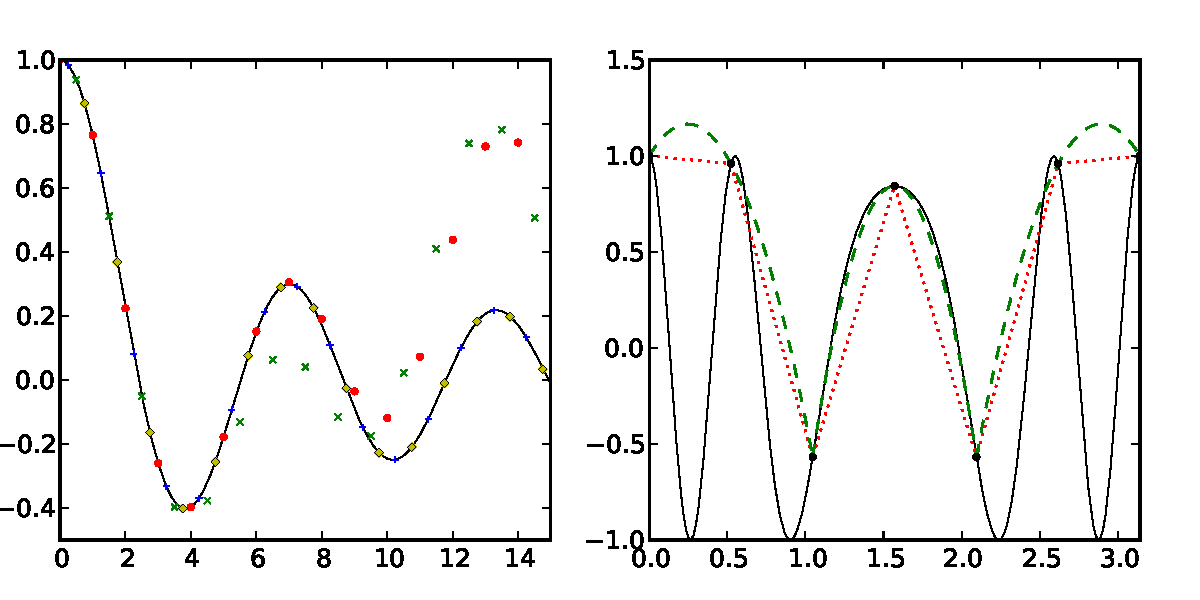
\includegraphics[width=\textwidth]{plots/bessel_int}
  \caption{Links: numerische Lösungen für das Besselintegral
    \eqref{eq:besselint}. Die durchgezogene schwarze Linie markiert
    die analytische Lösung. Blaue Plus-Symbole und gelbe Rauten
    markieren Trapez- bzw. Simpsonregel mit jeweils 20 Stützstellen.
    Rote Punkte und grüne Kreuze markieren dieselben Quadraturformeln,
    aber mit nur 6 Stützstellen. Rechts: in schwarz ist der Integrand
    von \eqref{eq:besselint} für $x=12$ dargestellt. Die schwarzen
    Punkte markieren darauf die 6 Stützstellen, durch die das Integral
    abgeschätzt werden soll. Rot gepunktet sind die linearen
    Näherungen, die in der Trapezregel integriert werden, grün
    gestrichelt die quadratischen Näherungen der zusammengesetzten
    Simpsonregel. Es ist klar, dass diese keine zufriedenstellende
    Auflösung des Integrals liefern können.}
  \label{fig:bessel_int}
\end{figure}

Als Beispiel für die numerische Integration soll uns noch einmal die
Besselfunktion erster Ordnung $J_\nu(x)$ dienen, also die Lösung der
Besselschen Differentialgleichung. Wie man durch Einsetzen in die
Differentialgleichung "`leicht"' sieht, ist $J_0(x)$ gegeben durch das
bestimmte Integral
\begin{equation}
  \label{eq:besselint}
  J_0(x) = \frac{1}{\pi} \int_0^\pi  \cos(x\sin(\tau))\,d\tau,
\end{equation}
das wir numerisch mit Hilfe der zusammengesetzten Trapez- und
Simpsonregel berechnen wollen. Wie Abbildung~\ref{fig:bessel_int}
links zeigt, gelingt dies mit nur 20 Stützpunkten recht
zufriedenstellend, sechs Stützpunkte allerdings ist für beide Regeln
nicht ausreichend. Zum Vergleich: die numerische Lösung der
Differentialgleichung mit dem Verfahren dritter Ordnung benötigt
dreihundert Stützpunkte, liefert aber auch eine Abschätzung der
Funktion an jedem Stützpunkt, während das Integral für jeden Punkt neu
gelöst werden muss.

Der Grund, dass sechs Stützstellen nicht ausreichen, ist im Prinzip
derselbe, wie wir ihn schon bei Abbildung~\ref{fig:num_diff} gesehen
haben: mit nur sechs Stützstellen lassen sich bei höheren $x$ die
Schwingungen nicht mehr auflösen, siehe Abbildung~\ref{fig:bessel_int}
rechts. Dies lässt sich auch durch das Verfahren höherer Ordnung nicht
korrigieren, sondern nur durch eine hinreichend kleine
Schrittweite. In diesem Fall sollte $h \ll 2\pi/x$ bzw. $N \gg x/2$
sein, so dass
\begin{equation}
  \abs{x\left(\sin(\tau + h) - \sin(\tau)\right)} \approx x h
  \abs{cos(\tau)} \ll 2\pi,
\end{equation}
damit der äußere Cosinus ausreichend aufgelöst wird.  Für größere $x$
als im Graphen gezeigt wird also auch $N=20$ nicht ausreichend sein.

\subsection{\keyword{Romberg-Integration}}
\index{Integration>Romberg-}

Ist $f\in C^{2k+2}([a,b])$ und
\begin{equation}
  T_f(h) = h\left(\frac{f(a)}{2} + \sum_{i=1}^{(b-a)/h - 1} f(a + i h) +
    \frac{f(b)}{2}\right) + \O(h^2)
\end{equation}
die (zusammengesetzte) Trapezformel zur Schrittweite $h$, so gilt die
\emph{\keyword{Euler-McLaurin-Summenformel}}
\begin{equation}
  T_f(h) = \int_a^b f(x)\,dx + \sum_{i=1}^k h^{2i}\alpha_i + \O(h^{2k-2})
\end{equation}
mit
\begin{equation}
  \alpha_i = \frac{b_{2i}}{(2i)!}\left(f^{(2i-1)}(b) - f^{(2i-1)}(a)\right).
\end{equation}
$b_{2i}$ bezeichnet dabei die Bernoullizahlen, die $\alpha_i$ hängen also
nicht von $h$ ab. 

In anderen Worten bedeutet das, dass sich der die Trapezregel in einer
Umgebung der 0 wie ein Polynom in $h^2$ verhält!  Damit können wir --
sofern wir die Werte $\alpha_i$ bestimmen können -- durch Auswerten
des Polynoms bei $h=0$, also bei unendlich kleiner Schrittweite, das
gesuchte Integral bis auf einen Fehler der Ordnung $\O(h^{2k-2})$
ausrechnen.

Für $b-a$-periodische $C^\infty$-Funktionen sind offenbar alle
$\alpha_i=0$, daher strebt die Trapezformel $T_f(h)$ für diese
schneller als jede Potenz von $h$ gegen das gesuchte Integral.

Für nichtperiodische Funktionen kann man im allgemeinen die $\alpha_i$
nicht analytisch bestimmen, weil das die Kenntnis hoher Ableitungen
erfordert. Um das gesuchte Polynom $T_f(h)$, und damit die $\alpha_i$,
trotzdem zu bestimmen, berechnet man zunächst $T_{i,0}=T_f(h_i)$ für
paarweise verschiedene Schrittweiten $h_0>h_1>\ldots>h_k>0$, und
bestimmt dann $T_f(h)$ als das interpolierende Polynom durch diese
Punkte. Dann kann man mit Hilfe des Neville-Aitken-Schemas das
interpolierende (Fehler-)Polynom in $h^2$ an der Stelle $0$ auswerten:
\begin{equation}
  \label{eq:richardson}
  T_{i,j} = T_{i+1,j-1} + \frac{T_{i+1,j-1} -
    T_{i,j-1}}{\frac{h_i^2}{h_{i+j}^2} -1}
  \quad\text{für}\; i=0(1)k-j, j=1(1)k.
\end{equation}
Dann gilt $T_{0,k} = T_f(0) + \O(h^{2k+2}) = \int_a^b f(x)\,dx +
\O(h^{2k+2})$. Eine solche Extrapolation von Schrittweiten $h>0$ auf
die Schrittweite Null heißt auch
\emph{\keyword{Richardson-Extrapolation}}.

Wählt man nun $h_i = \frac{b-a}{2^i}$, so vereinfacht sich
\eqref{eq:richardson} zu
\begin{equation}
  T_{ij} = T_{i+1,j-1} + \frac{T_{i+1,j-1} -
    T_{i,j-1}}{4^j - 1} = \frac{4^j T_{i+1,j-1} -
    T_{i,j-1}}{4^j - 1},
\end{equation}
was als \emph{Romberg-Integration} bezeichnet wird. Diese Wahl
der Schrittweiten hat auch den Vorteil, dass die Summe für $h_i$ bei
der Berechnung von $h_{i+1}$ wiederverwendet werden kann:
\begin{equation}
  T_f(h_{i+1}) = \frac{1}{2} T_f(h_i) +
  h_{i+1}\sum_{l=0}^{2^i-1} f\left(a + h_i\left(l
      + \frac{1}{2}\right)\right)
\end{equation}
Da sich der Aufwand für die Berechnung aller $T_f(h_i)$ mit jeder
Stufe verdoppelt, ist der Gesamtaufwand nicht wesentlich größer als
der Aufwand zur Berechnung der niedrigsten Stufe $T_f(h_k)$ alleine,
bei deutlicher Verbesserung der
Fehlerabschätzung. Codebeispiel~\ref{lst:romberg} am Ende des Kapitels
zeigt eine einfache, aber effiziente Implementation des
Rombergverfahrens mit Hilfe von SciPy. Alternativ bietet auch SciPy
selber eine Implementation des Verfahrens,
\scipy{scipy.integrate.romberg(f, a, b)}.

\lstinputlisting[style=floating,firstline=10,
caption={Romberg-Integration von $4(1+x^2)^{-1}$. Das Programm
  berechnet $\pi$ auf 16 Stellen genau.},
label=lst:romberg]{romberg.py}
\afterpage{\clearpage}
  
\subsection{Beispiel: Fehlerintegral}

Als Beispiel für die Romberg-Integration ist das Besselintegral aus
dem vorherigen Abschnitt wenig geeignet, da die zu integrierende
Funktion $b-a$-periodisch und $C^\infty$ ist. Dadurch konvergiert
bereits die einfache Trapezregel schneller als jedes Polynom, und
bereits mit nicht sehr kleinen Schrittweiten erreicht die Trapezregel
Maschinengenauigkeit. Da andererseits die Schrittweite wie beschrieben
hinreichend klein sein muss, bleibt nicht genügend Raum, um durch
Extrapolation noch etwas zu verbessern. 

\begin{figure}
  \centering
  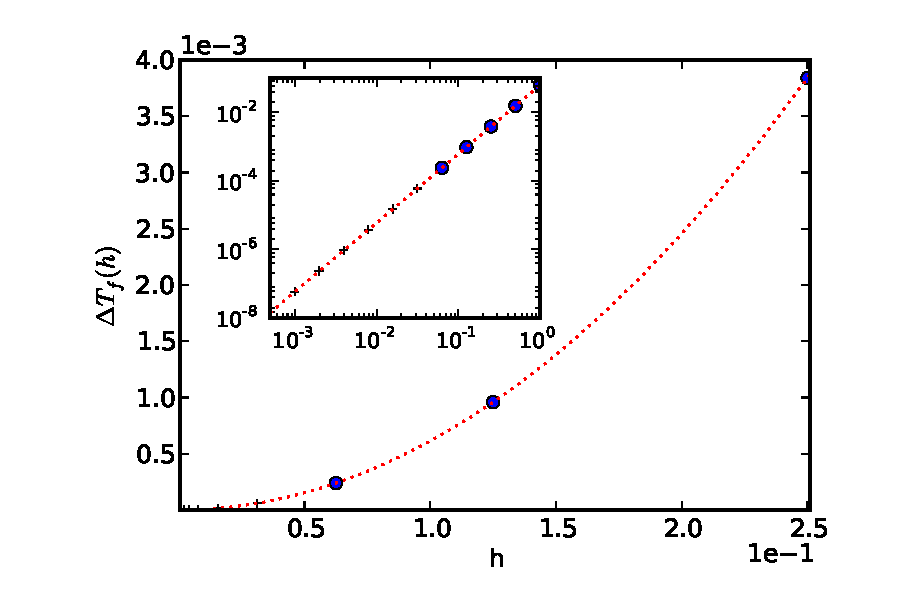
\includegraphics[width=0.75\textwidth]{plots/romberg}
  \caption{Romberg-Integration am Beispiel von $\int_0^1 e^{-x^2}\,dx
    = \sqrt{\pi}\erf(1)/2 =: T_0$. Aufgetragen ist der Fehler $\Delta
    T_f(h) = T_f(h) - T_0$ als Funktion der Schrittweite $h$ (im Einschub
    in doppeltlogarithmischer Skala). Sowohl Kreuze also auch blaue
    Kreise markieren Berechnungen mit der Trapezregel. Durch die mit
    blauen Kreisen markierten Datenpunkte wurde dann das
    interpolierende Polynom bestimmt und rot gestrichelt
    eingezeichnet. Während der beste benutzte Datenpunkt eine
    Genauigkeit von etwa $6\cdot10^{-5}$ erreicht, hat der
    extrapolierte Wert eine Genauigkeit von $3\cdot 10^{-16}$.  }
  \label{fig:romberg}
\end{figure}

Stattdessen wollen wir hier das Fehlerintegral $\int_0^1 e^{-x^2}\,dx
= \sqrt{\pi}\erf(1)/2$ verwenden (siehe Abbildung~\ref{fig:romberg}).
Dabei sind die Randwerte bereits der ersten Ableitung stark
verschieden, so dass $T_f(h)$ tatsächlich polynomielle Form hat und um
die Null herum in einer weiten Umgebung nahezu quadratisch ist. Daher
kann die Extrapolation den Fehler signifikant senken.  Im Beispiel
werden Schrittweiten der Trapezregel von 1 bis $1/16$ betrachtet. Bei
Schrittweite $1/16$ beträgt der Fehler der Trapezregel noch etwa
$6,0\cdot 10^{-5}$, während das Integral durch die Extrapolation von 5
Datenpunkten das Integral bis auf $3,3\cdot 10^{-16}$ korrekt
bestimmt, also Maschinengenauigkeit.

\subsection{\keyword{Gauß-Quadratur}}
\index{Integration>Gauß-Quadratur}

Bis jetzt hatten wir uns vor allem mit äquidistanten oder aber ganz
freien Gittern beschäftigt. Wenn aber die zu integrierende Funktion
analytisch gegeben ist, so können wir die Stützpunkte frei
wählen. Welche Stützpunkte sind dann optimal? Bei der Gauß-Quadratur
suchen wir Stützstellen $x_i$ und dazugehörige Gewichte $\alpha_i$, so
dass für Polynome $f$ mit möglichst hohem Grad noch
\begin{equation}
  \int_{-1}^1 f(x)\, dx = I_n f := \sum_{i=1}^n \alpha_i f(x_i)
\end{equation}
gilt, also dies Polynome exakt integriert werden. Die feste Wahl der
Integralgrenzen $a=-1$ und $b=1$ ist dabei keine Einschränkung, weil
jedes endliche Integral auf diesen Bereich transformiert werden kann:
\begin{equation}
  \int_a^b f(x)\, dx = \frac{(b-a)}{2} \int_{-1}^{1}f\bigl(
  \frac{a+b}{2} + x'\frac{b-a}{2}\bigr)\, dx'.
\end{equation}

Welchen Polynomgrad können wir so erreichen?  Auf der einen Seite
integrieren schon die Newton-Cotes-Formeln mit $n$ Stützstellen
Polynome bis Grad $n-1$ exakt. Auf der anderen Seite ist für das
Polynom $p(x) = \prod_{i=1}^n (x-x_i)^2$ jede Näherung $I_n p = 0$,
während offenbar $\int_{a}^{b} p(x)\,dx>0$. Daher kann es also kein
Verfahren geben, dass alle Polynome bis Grad $2n$ exakt
integriert. Ein Grad darunter, also $2n-1$ ist allerdings möglich, und
wird durch die Gauß-Quadratur erreicht.

Um ein Polynom $2n-1$ Grades eindeutig zu bestimmen, benötigen wir
$2n$ Stützstellen. Da wir aber nur $n$ Stützstellen benutzen wollen,
liegt es nahe, an diesen auch die Ableitungen einzubeziehen, was ein
Spezialfall der Hermite-Interpolation ist. Wie man leicht sieht, ist
\begin{equation}
  p(x) = \sum_{i=1}^n L_i^2(x)\Bigl\{f(x_i)\bigl[1-2L_i'(x_i)(x-x_i)\bigr] +
    f'(x_i)(x-x_i)\Bigr\}
\end{equation}
das gesuchte Polynom $2n-1$-Grades durch die Stützstellen $(x_i,
f(x_i), f'(x_i))$. $L_i$ bezeichnet die Lagrangepolynome aus Gleichung
\eqref{eq:lagrange}. Daraus ergibt sich die \emph{Hermite-Quadratur}
\begin{equation}
  \int_{-1}^1 f(x)\, dx \approx \int_{-1}^1 p(x)\, dx =
  \sum_{i=1}^{n} \alpha_i f(x_i) + \sum_{i=1}^{n} \beta_i f'(x_i)
\end{equation}
mit
\begin{equation}
  \alpha_i = \int_{-1}^1 L_i^2(x)\bigl[1-2L_i'(x_i)(x-x_i)\bigr]\,dx
  \quad\text{und}\quad
  \beta_i = \int_{-1}^1 L_i^2(x)(x-x_i)\, dx.
\end{equation}

\noindent Ziel ist nun, die Lage der Knoten $x_i$ so zu wählen, dass
die Ableitungen, die wir ja im allgemeinen gar nicht kennen, aus der
Näherungen entfallen:
\begin{equation}
  \label{eq:gaussortho}
  0 \stackrel{!}{=} \beta_i = \prod_{k\neq i}\frac{1}{x_i-x_k}
  \int_{-1}^1 L_i(x)\omega(x)\, dx,
\end{equation}
mit $\omega_n(x):=\prod_{i=1}^n(x-x_i)$. Da die $L_i$ eine Basis der
Polynome vom Grad $n-1$ bilden, bedeutet dies, dass $\omega_n$
bezüglich des üblichen Skalarprodukts $(f,\,g) = \int_{-1}^1
f(x)g(x)\,dx$ senkrecht auf dem Raum der Polynome vom Grad $n-1$
stehen muss. Mit $\beta_i=0$ vereinfacht sich außerdem
\begin{equation}
  \alpha_i = \int_{-1}^1 L_i^2(x)\,dx - 2L_i'(x_i)\beta_i
  = \int_{-1}^1 L_i^2(x)\, dx.
\end{equation}

Wir suchen also ein Polynom $\omega_n$ mit Höchstkoeffizient $1$ und
Grad $n$, dass senkrecht auf alles Polynomen vom Grad $n-1$ steht. Die
Nullstellen dieses Polynoms sind dann die gesuchten Stützstellen
$x_i$.  Die Existenz und Eindeutigkeit von $\omega_n$ kann man mit
Hilfe des Gram-Schmidt-Orthogonalisierungserfahrens konstruktiv
zeigen, dass wir später genauer kennenlernen werden. Die Idee ist
dabei, die Basisvektoren $\{1, x, x^2,\ldots\}$ schrittweise so zu
transformieren, dass sie senkrecht zu einanderstehen.

Dies ergibt, bis auf einen Vorfaktor, die
\emph{\keyword{Legendrepolynome}}, die rekursiv zum Beispiel so
berechnet werden können:
\begin{align}
  P_0(x) &= 1\nonumber\\
  P_1(x) &= x\nonumber\\
  P_n(x) &= \frac{1}{n}\Bigl((2n-1)xP_{n-1}(x) -
    (n-1)P_{n-2}(x)\Bigr).
\end{align}
{\samepage Die Nullstellen der ersten dieser Polynome und die
zugehörigen Gewichte sind
\begin{center}
  \renewcommand{\arraystretch}{1.2}
  \begin{tabular}{r|l|l}
    Grad & Nullstelle & Gewicht\\
    \hline\hline
    1    & $x_0=0$         & $\alpha_0=2$\\
    \hline
    2    & $x_{0,1} = \pm \sqrt{\nicefrac{1}{3}}$ &
    $\alpha_{0,1} = 1$ \\
    \hline
    3    & $x_{0,2} =  \pm \sqrt{\nicefrac{3}{5}}$ &
    $\alpha_{0,2}=\nicefrac{5}{9}$\\
    {}   & $x_1 =  0$                             &
    $\alpha_1=\nicefrac{8}{9}$\\
  \end{tabular}
\end{center}}
In SciPy implementiert \scipy{scipy.integrate.fixed_quad(f, a, b,
  n=5)} die Gauß-Quadratur mit den Nullstellen der
Legendrepolynome. \argd{n} gibt dabei die Anzahl der Stützstellen an,
die benutzt werden sollen.

Um andere Gauß-Quadraturen zu entwickeln, kann man gewichtete
Skalarprodukte betrachten. Wir definieren
\begin{equation}
  (f,g)_w := \int_{-1}^1 f(x)g(x)w(x)\, dx
\end{equation}
als das zur Gewichtsfunktion $w(x)>0$ gehörige Skalarprodukt. Dies
ändert unsere Orthogonalitätsbeziehung \eqref{eq:gaussortho} in
\begin{equation}
  0 \stackrel{!}{=} (L_i,\omega)_w = \int_{-1}^1 L_i(x)\omega(x)w(x)\, dx.
\end{equation}
Wenn wir die ursprüngliche Hermite-Interpolation beibehalten wollen,
bedeutet dies, dass wir auch das Zielintegral entsprechend anpassen
müssen, also nun
\begin{equation}
  \int_{-1}^1 f(x) w(x)\, dx \approx \int_{-1}^1 p(x) w(x)\, dx
  \sum_{i=1}^{n} \alpha_i f(x_i) + \sum_{i=1}^{n} \beta_i f'(x_i)
\end{equation}
berechnen mit
\begin{equation}
  \alpha_i = \int_{-1}^1 L_i^2(x)w(x)\, dx.
\end{equation}

Die Legendrepolynome bzw.\ deren Nullstellen gehören also zur
Gewichtsfunktion $w(x)=1$. Die Gewichtsfunktion
$w(x)=\nicefrac{1}{\sqrt{1-x^2}}$ hingegen liefert als Stützstellen
die Nullstellen der Chebyshev-Polynome $T_n(x)$, vergleiche
\eqref{eq:chebyshev}. Die Gewichte sind in diesem Fall sehr einfach,
nämlich $\pi/n$. Um das offene Intervall $(-\infty,\infty)$ zu
betrachten, kann die Gewichtsfunktion $e^{-x^2}$ benutzt werden, zu
der die orthogonalen Polynome die Hermitepolynome sind.

Als letztes soll noch erwähnt werden, dass die Gauß-Quadratur für alle
Gewichtsfunktionen mit steigender Anzahl von Stützstellen gegen das
tatsächliche Integral konvergiert, im Gegensatz zun den
Newton-Cotes-Formeln.

\subsection{Unendliche Integrale und Singularitäten}

\begin{figure}
  \centering
  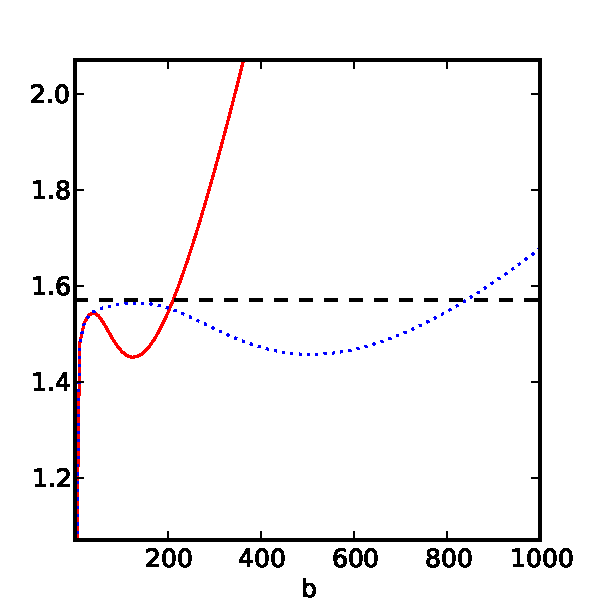
\includegraphics[width=0.5\textwidth]{plots/inf_int}
  \caption{Romberg-Verfahren für das Integral $\int_0^{b}
    \frac{1}{1+x^2}\, dx$, als Funktion von $b$. Die blau gepunktete
    Linie markiert die Ergebnisse des Verfahrens mit 128 Stützstellen,
    die rote durchgezogene Linie mit 32 Stützstellen. Die schwarz
    gestrichelte Linie markiert $\nicefrac{\pi}{2}$, also den
    Grenzwert des Integrals gegen unendlich. Eine Kombination von $b$
    und Anzahl Stützstellen zu finden, die diesen Grenzwert gut
    approximiert, ist also sehr schwierig.}
  \label{fig:inf_int}
\end{figure}

Alle genannten numerischen Integrationsverfahren lösen Integrale mit
Singularitäten nur schlecht. Unendliche Integrationsgrenzen sind, bis
auf die Gauß-Quadratur mit Hermitepolynomen, gar nicht möglich. In
ersterem Falle müssen sehr viele Stützpunkte in der Nähe der
Singularität liegen, im zweiten Fall muss das unendliche Integral
durch ein möglichst großes, endliches Intervall approximiert
werden. Allerdings ist es oft möglich, solche Probleme durch
Variablensubstitution zu umgehen.  So ist zum Beispiel
\begin{equation}
  \int_1^{\infty} \frac{f(x)}{x^2}dx \stackrel{z = \frac{1}{x}}{=}
  \int_0^1 f\left(\frac{1}{z}\right)dz.
\end{equation}
Fällt $f'(x)$ für große $x$ gegen $0$ ab, so dass $f$ gegen eine
Konstante strebt, dann ist die Ableitung von $f(1/z)$ gegen $0$
beschränkt, und die Funktion gut integrierbar. Im Unterschied zum
ursprünglichen Integral ist das neue Integral aber eigentlich und
damit mit den genannten Verfahren einfach zu lösen.

Als Beispiel soll die Berechnung von $\pi/2$ gemäß der Formel
\begin{equation}
  \frac{\pi}{2} = \int_0^{\infty} \frac{1}{1+x^2}\, dx
\end{equation}
dienen. Mit obiger Transformation folgt
\begin{equation}
  \int_0^{\infty} \frac{1}{1+x^2}\, dx
  = \int_0^1 \frac{1}{1+x^2}\, dx +  \int_0^1 \frac{1}{1+z^{-2}}z^{-2}\, dz
  = 2\int_0^1 \frac{1}{1+x^2}\, dx.
\end{equation}
Durch Romberg-Integration auf nur 32 Stützstellen kann der Ausdruck
auf der rechten Seite bis auf 14 Stellen genau ausgewertet
werden.

Abbildung~\ref{fig:inf_int} zeigt hingegen, was bei 32 bzw. 128
Stützstellen geschieht, wenn man stattdessen $\int_0^b
\frac{1}{1+x^2}\, dx$ für große $b$ mit Hilfe des Rombergverfahrens
bestimmt. Das Ergebnis hängt stark von der Integrationsgrenze $b$ ab,
und so ist es praktisch unmöglich, zu sagen, was der tatsächliche Wert
des Integrals für $b \rightarrow \infty$ ist. Durch Anpassen der
Anzahl der Stützpunkte an $b$ und damit Konstanthalten der
Schrittweite lässt sich zwar das Integral stabilisieren, trotzdem
müsste man mehrere Werte von $b$ mit hohen Anzahlen an Stützstellen
ausprobieren, um eine gute Näherung sicherzustellen. Im Beispiel
erreicht keines der beiden Extrema vorne mehr als 3 Stellen
Genauigkeit. Daher sollte man stets lieber versuchen, das Integral
durch Substitutionen auf eine endliche Form zu bringen.

\subsection{Mehrdimensionale Integration, \keyword{Monte-Carlo-Integration}}
\index{Integration>Monte-Carlo-}
\label{sec:mc}

Bis jetzt haben wir uns nur mit eindimensionalen Integralen
beschäftigt. Im Prinzip ist es nicht schwer, die obigen Verfahren auch
auf höhere Dimensionen zu erweitern, etwa die zusammengesetzte 
Mittelpunktsregel auf zwei Dimensionen:
\begin{equation}
  \int_a^b \int_c^d f(x, y)\, dx\, dy \approx
  \frac{(b-a)(d-c)}{NM} \sum_{i=0}^{N-1} \sum_{j=0}^{M-1}
  f\bigl(a + (b-a)\frac{i}{N}, c + (d-c)\frac{j}{N}\bigr).
\end{equation}
Hatte man allerdings bei einer hinreichend glatten Funktion bereits
mit hundert Stützstellen gute Ergebnisse erzielen können, benötigt man
nun etwa $100^2=10,000$ Stützstellen.  Mit steigender Anzahl der
Dimensionen wird dies schnell unmöglich zu handhaben. Für die
sogenannte \emph{Zustandssumme} eines Vielteilchensystems zum
Beispiel, einer zentralen Größe in der statistischen Physik, muss etwa
über allen Koordinaten des Phasenraums integriert werden.  Bei nur
hundert Teilchen entspräche das bereits 600 Dimensionen ($3$
Ortskoordinaten plus $3$ Geschwindigkeiten pro Teilchen). Sollten in
jeder dieser Koordinaten nur 2 Stützpunkte benutzt werden, wären
insgesamt trotzdem über $2^{600}= 4\cdot 10^{180}$ Stützpunkte zu
berücksichtigen! Für diesen exponentiellen Anstieg, der bei
praktischen allen hochdimensionalen Problemen auftritt, hat R.~Bellman
den Begriff "`Curse of dimensionality"' geprägt.

Um solche hochdimensionalen Integrale trotzdem annähern zu können,
kann man die Monte-Carlo-Integration einsetzen. Diese benutzt, dass
\begin{equation}
  \mean{\frac{1}{N} \sum_{i=1}^N f(\xi_i)} = \mean{f}_{V} =
  \int_{x\in V} f(x)\,dx / |V|,
\end{equation}
wobei $\xi_i$ verschiedene Ziehungen einer Zufallsvariablen sind, die
gleichverteilt in $V$ ist. $V$ ist dabei ein endliches Untervolumen
des $\RR^n$, $|V|$ sein Volumen. Daher lässt sich das Integral von $f$
als
\begin{equation}
  \int_{x\in V} f(x)\,dx \approx \frac{|V|}{N} \sum_{i=1}^N f(\xi_i)
\end{equation}
nähern, wobei $\xi_i$ hinreichend gute (Pseudo-)Zufallsvektoren aus
$V$ sein müssen. Wie diese generiert werden, ist Thema des nächsten
Kapitels. Was ist nun der Fehler dieser Näherung? Da die $\xi_i$ gemäß
Konstruktion unabhängig sind, lässt sich der Fehler gut mit Hilfe der
Standardabweichung $\sigma(f)$ abschätzen, und beträgt
$|V|\sigma(f)/\sqrt{N}$. Die Standardabweichung kennen wir im
allgemeinen nicht, können sie aber gemäß~\eqref{eq:varest} als
\begin{equation}
  \sigma^2(x) \approx \frac{1}{N-1} \left[\sum_{i=1}^N f(\xi_i)^2 -
    N\left(\sum_{i=1}^Nf(\xi_i)\right)^2\right]
\end{equation}
zusammen mit der Integration abschätzen.

Als SciPy-Code sieht eine Monte-Carlo-Integration noch einfacher als
die Trapezregel aus. Hier ein Code, der zweidimensional über
$[a,b]\times[c,d]$ integriert:
\begin{lstlisting}
from numpy.random import uniform

def montecarlo(f, a, b, c, d, N):
    volumen = (b-a)*(d-c)
    return volumen*sum(f(uniform(a,b,N), uniform(c,d,N)))/N
\end{lstlisting}

Da die Standardabweichung eine Konstante ist, fällt der Fehler der
Monte-Carlo-Integration im allgemeinen wie $\O(N^{-1/2})$. Im
Vergleich dazu fällt der Fehler der Trapezregel im eindimensionalen
wie $\O(N^{-2})$, sofern $f$ genügend glatt ist. Wenn man bei der
Trapezregel die Anzahl der Stützpunkte verdoppelt, dann muss man bei
der Monte-Carlo-Integration mehr als eine Größenordnung mehr Punkte
aufwenden, um dieselbe Verbesserung in der Genauigkeit zu erreichen!

Bei mehrdimensionalen Integralen sieht die Situation allerdings anders
aus. Bei der Trapezregel mit ingesamt $N$ Stützstellen entfallen pro
Dimension $N^{1/n}$ viele Stützstellen, wenn diese auf einem Würfel
gleichmässig in allen Dimensionen verteilt werden.  Die Genauigkeit
ist damit $\O(N^{-2/n})$.  Ab fünf Dimensionen ist damit die
Monte-Carlo-Integration der Trapezregel überlegen.  Ein anderer Fall,
in dem die Monte-Carlo-Integration der Trapezregel überlegen sein
kann, ist wenn die Funktion $f$ nicht genügend glatt oder nicht einmal
stetig ist.

\subsection{\texorpdfstring{Beispiel: Monte-Carlo-Integration von
    $\pi$}{Beispiel: Quasi-Monte-Carlo-Integration von pi}}

Als Beispiel soll diesmal eine andere Methode zur Bestimmung von
$\pi$ dienen, nämlich die Integration der charakteristischen Funktion
\begin{equation}
  \chi_{D^2}(x, y)=
  \begin{cases}
    1 & \text{falls}\; x^2 + y^2 < 1\\
    0 & \text{sonst}
  \end{cases}
\end{equation}
im Bereich $[-1,1]^2$. Das ergibt dann gerade den Kreisinhalt, also
\begin{equation}
  \int_{x\in[-1,1]}\int_{y\in[-1,1]}\chi_{D^2}(x, y)\,dx\,dy
  = \pi.
\end{equation}

\begin{figure}
  \centering
  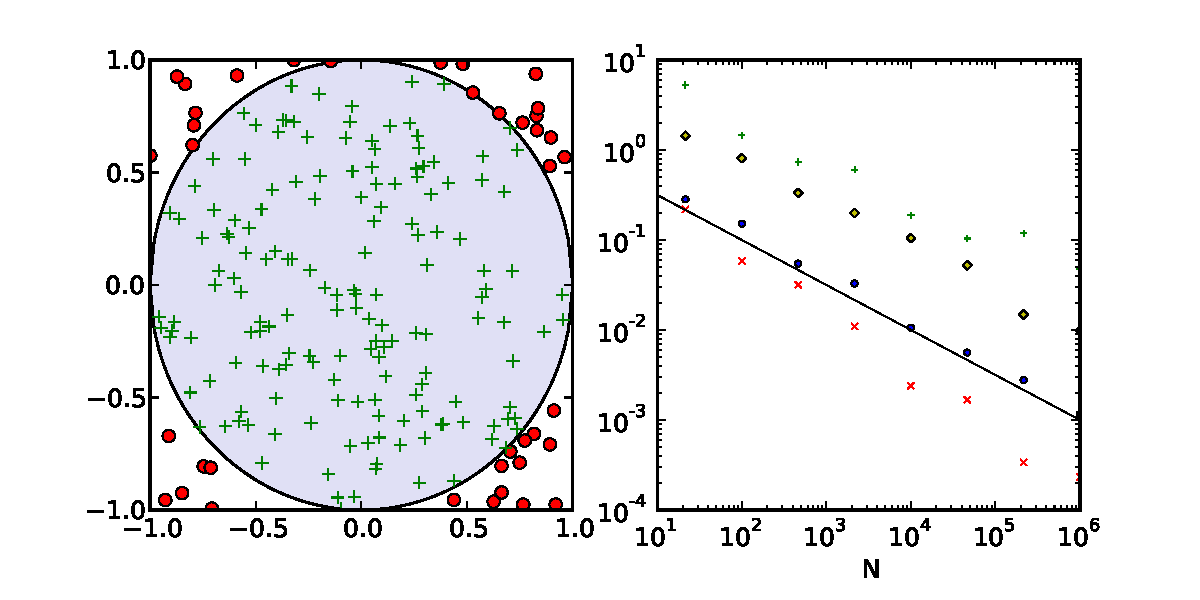
\includegraphics[width=\textwidth]{plots/pi}
  \caption{Links: Illustration der Monte-Carlo-Integration. Die
    Funktion $\chi_{D^2}$ wird über 200 zufällige Punkte (rote Kreise
    und grüne Kreuze) innerhalb $[-1,1]^2$ gemittelt. An den grünen
    Kreuzen ist $\chi_{D^2}=1$, für die roten Punkte ist es
    Null. Rechts: Genauigkeit der Integralnäherungen als Funktion der
    Anzahl der Stützstellen $N$.  Blaue Punkte markieren die mittlere
    Genauigkeit der zweidimensionalen Monte-Carlo-Integration wie
    links skizziert, die roten Kreuze die entsprechende
    Mittelpunktsregel. Gelbe Rauten und grüne Kreuze zeigen die
    Genauigkeiten von Monte-Carlo-Integration und Mittelpunktsregel
    für die 5-Kugel, bei der die Monte-Carlo-Integration schon klar
    überlegen ist. Die durchgezogene Linie entspricht einer Skalierung
    von $N^{-1/2}$, wie man sie für die Monte-Carlo-Integration
    erwartet.}
  \label{fig:pi}
\end{figure}

Abbildung~\ref{fig:pi} skizziert links die Monte-Carlo-Integration von
$\chi_{D^2}$, rechts zeigt sie gemessene Fehler bei
Monte-Carlo-Integration und Mittelpunktsregel. Dabei wurde neben
$\chi_{D^2}$ auch $\chi_{D^5}$ integriert, also das Volumen der
fünfdimensionalen Kugel ($8\pi^2/15$). Der Fehler der
Monte-Carlo-Integration ist jeweils als mittlerer Fehler von zwanzig
Aufrufen gemessen, wobei durch die große Anzahl von Abtastungen die
Schwankungen nicht sehr hoch sind.

Für das ursprüngliche, zweidimensionale Problem (blaue Punkte und rote
Kreuze) ist die Trapezregel überlegen, auch wenn sie in zwei
Dimensionen nicht die erwartete Skalierung mit $1/N$ erreicht. Das ist
zu erwarten, da die zu integrierende Funktion ja nicht stetig
ist. Auch der nichtmonotone Abstieg der Fehler ist durch die
Unstetigkeit und die Auflösung des Kreisrands bedingt. Beim
fünfdimensionalen Problem aber sieht es wie angekündigt anders aus,
hier ist die Monte-Carlo-Integration besser. Tatsächlich sind nicht
nur die mittleren Abweichungen kleiner als bei der Trapezregel,
sondern es ist sogar sehr unwahrscheinlich, ein ebenso schlechtes
Ergebnis zu erzielen. Für solche Integrale ist also die
Monte-Carlo-Methode in jedem Falle vorzuziehen.

\subsection{\keyword{Quasi-Monte-Carlo-Integration}}
\index{Integration>Quasi-Monte-Carlo-}

Bei der Monte-Carlo-Integration nutzen wir (Pseudo-)Zufallszahlen, um
durch zufällige Abtastung möglichst gut den mittleren Wert der zu
integrierenden Funktion zu bestimmen. Wie wir gesehen haben, sind im
Mehrdimensionalen Zufallszahlen zu diesem Zweck besser geeignet als
ein regelmäßiges Gitter --- das entspräche der ja der
Trapezregel. Aber sind Zufallszahlen optimal?

Tatsächlich nicht, denn etwa Abbildung~\ref{fig:optical_test} links
zeigt, dass Zufallszahlen nicht so homogen verteilt sind, wie man
annehmen würde. Dies ist kein Fehler des betrachteten
Zufallszahlengenerators, sondern ein prinzipielles Problem echter
Zufallssequenzen, die sogenannte \emph{\keyword{Diskrepanz}}. Unsere
Erwartung an eine Reihe von $N$ gleichverteilten Zufallszahlen ist,
dass jedes Intervall $[a,b]\subseteq [0,1]$ von etwa $(b-a)N$
Zufallszahlen getroffen wird. Dies ist aber bei echten Zufallszahlen
erst bei sehr großen $N$ der Fall. Das bedeutet, dass es bei der
Monte-Carlo-Integration immer Bereiche gibt, die von einer echten
Zufallsreihe über- oder unterrepräsentiert werden. Hat aber einer
dieser Bereiche einen großen Anteil am betrachteten Integral, führt
dies zu entsprechenden Fehlern.

\subsubsection{\keyword{Quasizufallszahlen}}

Anstelle von Zufallszahlen benutzt man daher für die
Monte-Carlo-Integration besser \emph{Quasizufallszahlen}, die nicht
mehr wirklich zufällig sind, sondern eine möglichst geringe Diskrepanz
bieten. Ziel ist es also, möglichst alle Bereiche mit genau so vielen
Zahlen abzudecken, wie man nach Gleichverteilung erwarten würde. Ein
Beispiel ist die \emph{\keyword{Halton-Folge}}, die eine Reihe mit
niedriger Diskrepanz im Wertebereich $[0,1]$ ist.

Um die Halton-Folge zu definieren, wählen wir für jede Dimension eine
andere Primzahl $p$ als Basis und schreiben die natürlichen Zahlen in
Basis $p$. Um daraus die gewünschte Zerlegung des Intervalls $[0,1]$
zu erhalten, benutzen wir einfach die Stellen der $p$-Darstellung als
Nachkommastellen, in umgekehrter Reihenfolge:
\begin{center}
  \begin{minipage}[t]{0.49\textwidth}
    \centering
    \begin{tabular}[t]{l|r|l|l}
      $n$ & binär & Stellenumkehr & Ergebnis\\\hline
      1 &   1 & ,1 & \nicefrac{1}{2}\\\hline
      2 &  10 & ,01 & \nicefrac{1}{4}\\
      3 &  11 & ,11 & \nicefrac{3}{4}
    \end{tabular}
  \end{minipage}
  \begin{minipage}[t]{0.49\textwidth}
    \centering
    \begin{tabular}[t]{l|r|l|l}
      $n$ & binär & Stellenumkehr & Ergebnis\\\hline
      4 & 100 & ,001 & \nicefrac{1}{8}\\
      5 & 101 & ,101 & \nicefrac{5}{8}\\
      6 & 110 & ,011 & \nicefrac{3}{8}\\
      7 & 111 & ,111 & \nicefrac{7}{8}
    \end{tabular}
  \end{minipage}
\end{center}
Für $p=3$ ergibt sich analog aus der ternären Darstellung
\begin{center}
  \begin{minipage}[t]{0.49\textwidth}
    \centering
    \begin{tabular}[t]{l|r|l|l}
      $n$ & ternär & Stellenumkehr & Ergebnis\\\hline
      1 &   1 & ,1 & \nicefrac{1}{3}\\
      2 &   2 & ,2 & \nicefrac{2}{3}\\\hline
      3 &  10 & ,01 & \nicefrac{1}{9}\\
      4 &  11 & ,11 & \nicefrac{4}{9}\\
    \end{tabular}
  \end{minipage}
  \begin{minipage}[t]{0.49\textwidth}
    \centering
    \begin{tabular}[t]{l|r|l|l}
      $n$ & ternär & Stellenumkehr & Ergebnis\\\hline
      5 &  12 & ,21 & \nicefrac{7}{9}\\
      6 &  20 & ,02 & \nicefrac{2}{9}\\
      7 &  21 & ,12 & \nicefrac{5}{9}\\
      8 &  22 & ,22 & \nicefrac{8}{9}
    \end{tabular}
  \end{minipage}
\end{center}
Die Umkehrung der Stellen hat den Vorteil, dass die $p^n$-tel
nacheinander möglichst gleichmäßig das Intervall füllen, was ja gerade
einer niedrigen Diskrepanz entspricht. Die sich ergebende Folge heißt
eine \emph{van der Corput-Folge}.

Die mehrdimensionale Halton-Folge ist dann die Folge, die aus der
Verschränkung einer van Corput-Folge für jede Dimension entsteht. Bei
zwei Dimensionen mit Basen 2 und 3 ergibt sich also
\begin{equation}
  \left(\nicefrac{1}{2}, \nicefrac{1}{3}\right),
  \left(\nicefrac{1}{4}, \nicefrac{2}{3}\right),
  \left(\nicefrac{3}{4}, \nicefrac{1}{9}\right),
  \left(\nicefrac{1}{8}, \nicefrac{4}{9}\right),
  \left(\nicefrac{5}{8}, \nicefrac{7}{9}\right),
  \left(\nicefrac{3}{8}, \nicefrac{2}{9}\right),
  \left(\nicefrac{7}{8}, \nicefrac{5}{9}\right),\ldots
\end{equation}

Die folgende Routine berechnet die ersten $N$ Glieder der van der
Corput-Folge zur Basis $p$. Dazu wird solange von den natürlichen
Zahlen $1,2,\ldots,N$ die unterste Stelle abgezogen und mit der
reziproken Potenz auf das Ergebnis addiert, bis alle Stellen von auch
der höchsten Zahl, $N$, bearbeitet wurden:
\begin{lstlisting}
from numpy import *
def vanderCorput(N, p):
    # zu wandelnde Zahlen
    numbers = arange(1,int(N)+1)
    # bitumgekehrtes Ergebnis
    result = zeros(N)
    # Wert der aktuellen, inversen Stelle
    frac = 1.0 / p

    # solange die groesste Zahl noch Stellen hat
    while numbers[-1] > 0:
        # unterste Stelle abschneiden
        digit = numbers % p
        numbers /= p
        # ... und zum Ergebnis hinzufuegen
        result += frac*digit
        frac /= p

    return array(result)
\end{lstlisting}
Um eine Monte-Carlo-Integration mit Quasizufallszahlen durchzuführen,
müssen im Beispielcode zum Abschnitt~\ref{sec:mc} lediglich die
Aufrufe von \lstinline!uniform(a,b,N)! durch
\lstinline!a + (b-a)*vanderCorput(N, p)! ersetzt werden. Üblicherweise
wählt man dabei $p=2$ für die erste Dimension, $p=3$ für die zweite,
und so weiter.

\subsection{\texorpdfstring{Beispiel: Quasi-Monte-Carlo-Integration von $\pi$}{Beispiel: Quasi-Monte-Carlo-Integration von pi}}

\begin{figure}
  \centering
  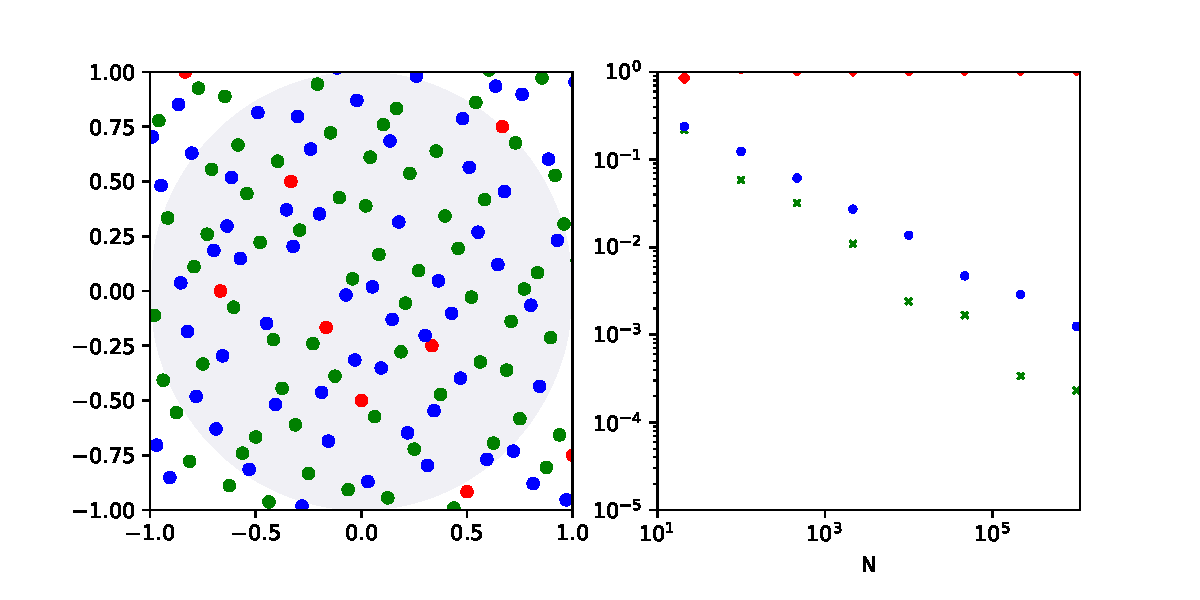
\includegraphics[width=\textwidth]{plots/quasirandom}
  \caption{Quasi-Monte-Carlo-Integration von $\pi$. Wie in
    Abbildung~\ref{fig:pi} sind links die aus der Halton-Folge
    gezogenen Punkte dargestellt, wobei die ersten zehn Punkte rot
    gefärbt sind, die nächsten hundert Punkte blau und die restlichen
    grün. Auf der rechten Seite sind die Ergebnisse der Integration zu
    sehen, wobei blaue Kreise die Monte-Carlo-Integration mit
    Pseudozufallszahlen angeben, grüne Kreuze die Trapezregel und rote
    Diamanten die Quasi-Monte-Carlo-Integration.}
  \label{fig:qmc}
\end{figure}

Abbildung~\ref{fig:qmc} zeigt nochmals die Integration von $\pi$ mit
Hilfe der Monte-Carlo-Integration, allerdings diesmal nicht mit
Pseudozufallszahlen, sondern der Halton-Folge, also
Quasizufallszahlen. Wie man gut sieht, sind die Quasizufallszahlen
scheinbar zufällig, aber sehr viel homogener als echte oder
Pseudozufallszahlen über das Quadrat verteilt, insbesondere auch schon
bei niedrigen Anzahlen von Punkten.  Die Integration mit
Quasizufallszahlen wird kurz als \emph{Quasi}-Monte-Carlo-Integration
bezeichnet, und ist für die unstetige Indikatorfunktion nicht nur der
Monte-Carlo-Integration mit Zufallszahlen überlegen, sondern auch der
Trapezregel.

%%% Local Variables: 
%%% mode: latex
%%% TeX-master: "padc.tex"
%%% TeX-PDF-mode: t
%%% End: 
